\documentclass{standalone}
\usepackage{tikz}
\usetikzlibrary{patterns, positioning}


\begin{document}
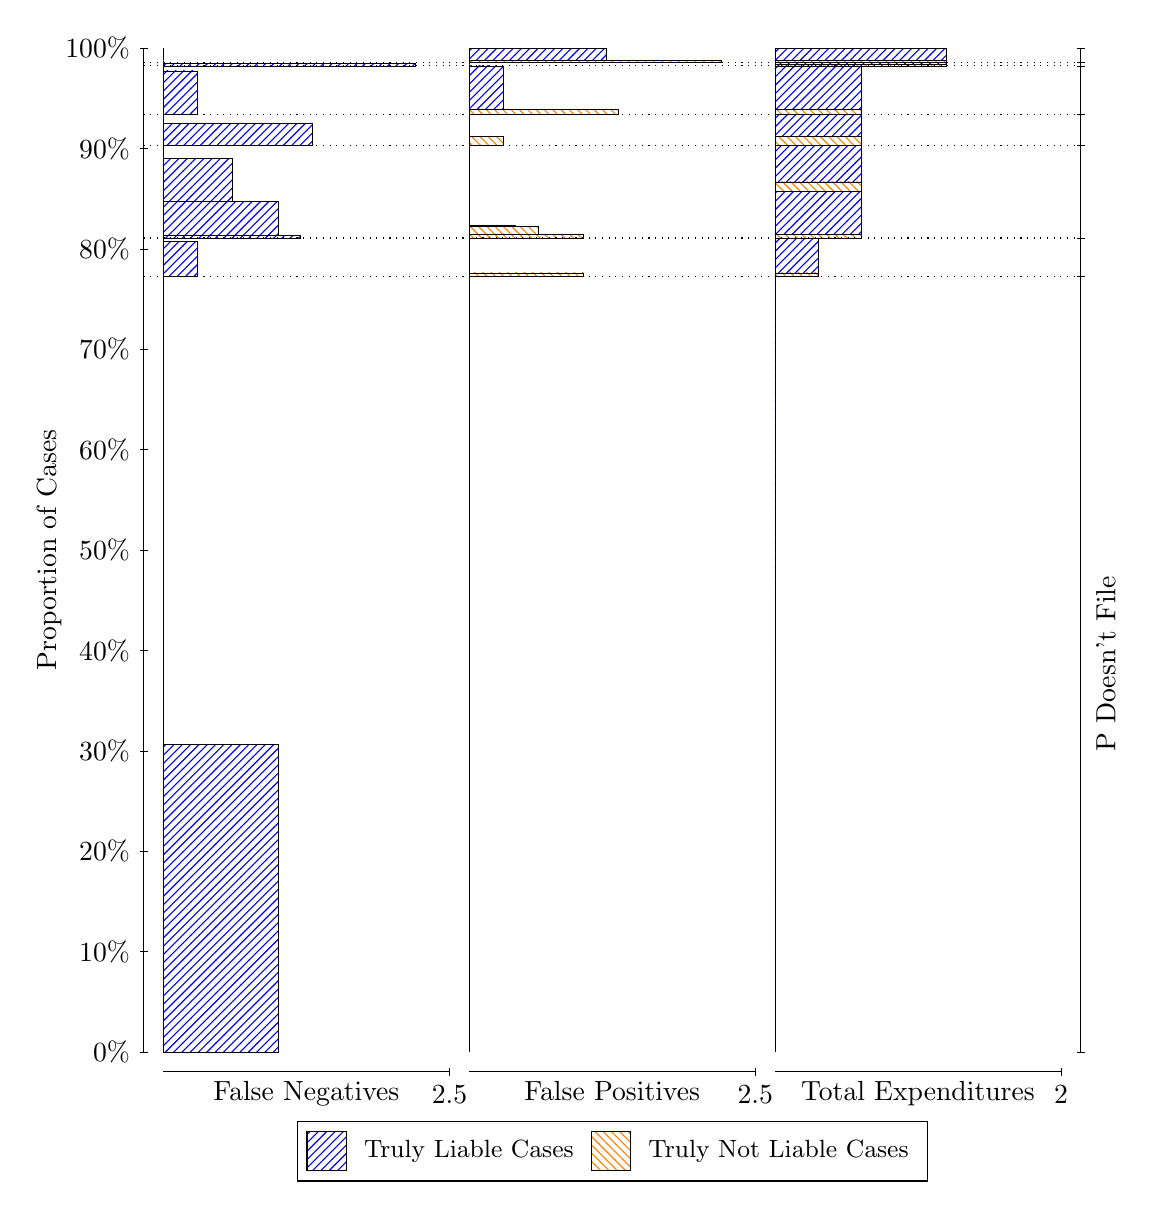
\begin{tikzpicture}
\draw[black, very thin] (1.5,1.75) -- (1.5,14.5);
\node[rotate=90, text=black, anchor=center] at (0.3, 8.125) {Proportion of Cases};
\draw[black, very thin] (1.45,1.75) -- (1.55,1.75);
\node[text=black, anchor=east] at (1.45, 1.75) {0\%};
\draw[black, very thin] (1.45,3.025) -- (1.55,3.025);
\node[text=black, anchor=east] at (1.45, 3.025) {10\%};
\draw[black, very thin] (1.45,4.3) -- (1.55,4.3);
\node[text=black, anchor=east] at (1.45, 4.3) {20\%};
\draw[black, very thin] (1.45,5.575) -- (1.55,5.575);
\node[text=black, anchor=east] at (1.45, 5.575) {30\%};
\draw[black, very thin] (1.45,6.85) -- (1.55,6.85);
\node[text=black, anchor=east] at (1.45, 6.85) {40\%};
\draw[black, very thin] (1.45,8.125) -- (1.55,8.125);
\node[text=black, anchor=east] at (1.45, 8.125) {50\%};
\draw[black, very thin] (1.45,9.4) -- (1.55,9.4);
\node[text=black, anchor=east] at (1.45, 9.4) {60\%};
\draw[black, very thin] (1.45,10.675) -- (1.55,10.675);
\node[text=black, anchor=east] at (1.45, 10.675) {70\%};
\draw[black, very thin] (1.45,11.95) -- (1.55,11.95);
\node[text=black, anchor=east] at (1.45, 11.95) {80\%};
\draw[black, very thin] (1.45,13.225) -- (1.55,13.225);
\node[text=black, anchor=east] at (1.45, 13.225) {90\%};
\draw[black, very thin] (1.45,14.5) -- (1.55,14.5);
\node[text=black, anchor=east] at (1.45, 14.5) {100\%};

\draw[black, very thin] (13.4,1.75) -- (13.4,14.5);
\draw[black, very thin] (13.35,1.75) -- (13.45,1.75);
\node[anchor=west] at (13.35, 1.75) {};
\draw[black, very thin] (13.35,11.603) -- (13.45,11.603);
\node[anchor=west] at (13.35, 11.603) {};
\draw[black, very thin] (13.35,12.087) -- (13.45,12.087);
\node[anchor=west] at (13.35, 12.087) {};
\draw[black, very thin] (13.35,13.264) -- (13.45,13.264);
\node[anchor=west] at (13.35, 13.264) {};
\draw[black, very thin] (13.35,13.658) -- (13.45,13.658);
\node[anchor=west] at (13.35, 13.658) {};
\draw[black, very thin] (13.35,14.273) -- (13.45,14.273);
\node[anchor=west] at (13.35, 14.273) {};
\draw[black, very thin] (13.35,14.317) -- (13.45,14.317);
\node[anchor=west] at (13.35, 14.317) {};
\draw[black, very thin] (13.35,14.5) -- (13.45,14.5);
\node[anchor=west] at (13.35, 14.5) {};

\draw[black, very thin, pattern color=blue, pattern=north east lines] (1.75,1.75) rectangle (3.2033,5.6581);
\draw[black, very thin, pattern color=orange, pattern=north west lines] (1.75,5.6581) rectangle (1.75,11.603);
\draw[black, very thin, pattern color=blue, pattern=north east lines] (1.75,11.603) rectangle (2.186,12.047);
\draw[black, very thin, pattern color=orange, pattern=north west lines] (1.75,12.047) rectangle (1.75,12.087);
\draw[black, very thin, pattern color=blue, pattern=north east lines] (1.75,12.087) rectangle (3.494,12.116);
\draw[black, very thin, pattern color=blue, pattern=north east lines] (1.75,12.116) rectangle (3.2033,12.551);
\draw[black, very thin, pattern color=blue, pattern=north east lines] (1.75,12.551) rectangle (2.622,13.1);
\draw[black, very thin, pattern color=orange, pattern=north west lines] (1.75,13.1) rectangle (1.75,13.264);
\draw[black, very thin, pattern color=blue, pattern=north east lines] (1.75,13.264) rectangle (3.6393,13.541);
\draw[black, very thin, pattern color=orange, pattern=north west lines] (1.75,13.541) rectangle (1.75,13.658);
\draw[black, very thin, pattern color=blue, pattern=north east lines] (1.75,13.658) rectangle (2.186,14.209);
\draw[black, very thin, pattern color=orange, pattern=north west lines] (1.75,14.209) rectangle (1.75,14.273);
\draw[black, very thin, pattern color=blue, pattern=north east lines] (1.75,14.273) rectangle (4.9473,14.3);
\draw[black, very thin, pattern color=orange, pattern=north west lines] (1.75,14.3) rectangle (1.75,14.317);
\draw[black, very thin, pattern color=orange, pattern=north west lines] (1.75,14.317) rectangle (1.75,14.344);
\draw[black, very thin, pattern color=blue, pattern=north east lines] (1.75,14.344) rectangle (1.75,14.5);
\draw[black, very thin, pattern color=orange, pattern=north west lines] (5.6333,1.75) rectangle (5.6333,7.6948);
\draw[black, very thin, pattern color=blue, pattern=north east lines] (5.6333,7.6948) rectangle (5.6333,11.603);
\draw[black, very thin, pattern color=orange, pattern=north west lines] (5.6333,11.603) rectangle (7.0867,11.643);
\draw[black, very thin, pattern color=blue, pattern=north east lines] (5.6333,11.643) rectangle (5.6333,12.087);
\draw[black, very thin, pattern color=orange, pattern=north west lines] (5.6333,12.087) rectangle (7.0867,12.13);
\draw[black, very thin, pattern color=orange, pattern=north west lines] (5.6333,12.13) rectangle (6.5053,12.238);
\draw[black, very thin, pattern color=orange, pattern=north west lines] (5.6333,12.238) rectangle (6.2147,12.251);
\draw[black, very thin, pattern color=blue, pattern=north east lines] (5.6333,12.251) rectangle (5.6333,13.264);
\draw[black, very thin, pattern color=orange, pattern=north west lines] (5.6333,13.264) rectangle (6.0693,13.382);
\draw[black, very thin, pattern color=blue, pattern=north east lines] (5.6333,13.382) rectangle (5.6333,13.658);
\draw[black, very thin, pattern color=orange, pattern=north west lines] (5.6333,13.658) rectangle (7.5227,13.722);
\draw[black, very thin, pattern color=blue, pattern=north east lines] (5.6333,13.722) rectangle (6.0693,14.273);
\draw[black, very thin, pattern color=orange, pattern=north west lines] (5.6333,14.273) rectangle (5.6333,14.291);
\draw[black, very thin, pattern color=blue, pattern=north east lines] (5.6333,14.291) rectangle (5.6333,14.317);
\draw[black, very thin, pattern color=orange, pattern=north west lines] (5.6333,14.317) rectangle (8.8307,14.344);
\draw[black, very thin, pattern color=blue, pattern=north east lines] (5.6333,14.344) rectangle (7.3773,14.5);
\draw[black, very thin, pattern color=orange, pattern=north west lines] (9.5167,1.75) rectangle (9.5167,7.6948);
\draw[black, very thin, pattern color=blue, pattern=north east lines] (9.5167,7.6948) rectangle (9.5167,11.603);
\draw[black, very thin, pattern color=orange, pattern=north west lines] (9.5167,11.603) rectangle (10.062,11.643);
\draw[black, very thin, pattern color=blue, pattern=north east lines] (9.5167,11.643) rectangle (10.062,12.087);
\draw[black, very thin, pattern color=orange, pattern=north west lines] (9.5167,12.087) rectangle (10.607,12.13);
\draw[black, very thin, pattern color=blue, pattern=north east lines] (9.5167,12.13) rectangle (10.607,12.679);
\draw[black, very thin, pattern color=orange, pattern=north west lines] (9.5167,12.679) rectangle (10.607,12.8);
\draw[black, very thin, pattern color=blue, pattern=north east lines] (9.5167,12.8) rectangle (10.607,13.264);
\draw[black, very thin, pattern color=orange, pattern=north west lines] (9.5167,13.264) rectangle (10.607,13.382);
\draw[black, very thin, pattern color=blue, pattern=north east lines] (9.5167,13.382) rectangle (10.607,13.658);
\draw[black, very thin, pattern color=orange, pattern=north west lines] (9.5167,13.658) rectangle (10.607,13.722);
\draw[black, very thin, pattern color=blue, pattern=north east lines] (9.5167,13.722) rectangle (10.607,14.273);
\draw[black, very thin, pattern color=orange, pattern=north west lines] (9.5167,14.273) rectangle (11.697,14.291);
\draw[black, very thin, pattern color=blue, pattern=north east lines] (9.5167,14.291) rectangle (11.697,14.317);
\draw[black, very thin, pattern color=orange, pattern=north west lines] (9.5167,14.317) rectangle (11.697,14.344);
\draw[black, very thin, pattern color=blue, pattern=north east lines] (9.5167,14.344) rectangle (11.697,14.5);
\draw[black, dotted] (1.5,11.603) -- (13.4,11.603);
\draw[black, dotted] (1.5,12.087) -- (13.4,12.087);
\draw[black, dotted] (1.5,13.264) -- (13.4,13.264);
\draw[black, dotted] (1.5,13.658) -- (13.4,13.658);
\draw[black, dotted] (1.5,14.273) -- (13.4,14.273);
\draw[black, dotted] (1.5,14.317) -- (13.4,14.317);
\draw[black, very thin] (1.75,1.5) -- (5.3833,1.5);
\node[text=black, anchor=north] at (3.5667, 1.5) {False Negatives};
\draw[black, very thin] (5.3833,1.45) -- (5.3833,1.55);
\node[text=black, anchor=north] at (5.3833, 1.45) {2.5};

\draw[black, very thin] (5.6333,1.5) -- (9.2667,1.5);
\node[text=black, anchor=north] at (7.45, 1.5) {False Positives};
\draw[black, very thin] (9.2667,1.45) -- (9.2667,1.55);
\node[text=black, anchor=north] at (9.2667, 1.45) {2.5};

\draw[black, very thin] (9.5167,1.5) -- (13.15,1.5);
\node[text=black, anchor=north] at (11.333, 1.5) {Total Expenditures};
\draw[black, very thin] (13.15,1.45) -- (13.15,1.55);
\node[text=black, anchor=north] at (13.15, 1.45) {2};

\node[text=black, centered, rotate=90] at (13.72, 6.6765) {P Doesn't File};







\draw (7.449999999999999,1.5) node[draw=none] (baseCoordinate) {};
\begin{scope}[align=center]
        \matrix[scale=0.5, draw=black, below=0.5cm of baseCoordinate, nodes={draw}, column sep=0.1cm]{
            \node[rectangle, draw, minimum width=0.5cm, minimum height=0.5cm, pattern color=blue, pattern=north east lines] {}; &
            \node[draw=none, font=\small, text=black] (B) {Truly Liable Cases}; &
            \node[rectangle, draw, minimum width=0.5cm, minimum height=0.5cm, pattern color=orange, pattern=north west lines] {}; &
            \node[draw=none, font=\small, text=black] (B) {Truly Not Liable Cases}; \\
            };
\end{scope}

\end{tikzpicture}
\end{document}